\section{Optimisation}\label{sec:optimisation}
In this section, we study optimisation with fixed NPFs, i.e., a setting in which $\ip{\partial \phi,v}=0$. Here, we are interested in learning $\hat{y}_{\Theta}(x)=\ip{\phi_{x,\Theta'}, v_{\Theta}}$, where $\Theta'\in\R^{d_{net}}$ is a fixed parameter that is non-trainable and $\phi_{x,\Theta'}$ is the corresponding fixed NPF, and optimising with GD boils down to learning the NPVs $v_{\Theta}$. In order to separate the NPFs from the NPVs, we use the DGN framework, wherein, there is a separate gating network to hold $\Theta'$, i.e, the fixed NPFs and $\Theta$ is held in a different network known as the value network. We study the following two interesting cases of fixed NPFs:\\
\textbf{Case $1.$} \emph{Random NPFs} obtained from the gates of a randomly initialised (a random $\Theta'$) neural network. We demonstrate that networks trained with fixed random NPFs can generalise.\\
\textbf{Case $2.$} We first train a DNN (with ReLU) till $T$ epochs. We then obtain the NPFs by letting $\Theta'=\Theta_T$. We then reset the weights $\Theta$ by initialising them randomly, and learn the NPVs again by training $\Theta$. We show in experiments there is only a marginal decrease in performance when learning with fixed learnt NPFs.
\FloatBarrier
\begin{table}[h] 
\begin{minipage}{0.75\columnwidth}
\resizebox{\columnwidth}{!}{
\begin{tabular}{|l|l|l|}\hline
Layer& Gating Network (NPF)&Value Network (NPV)\\\hline 
Input & $z_{x,\Tg_t}(0)=x$ &$z_{x,\Theta_t}(0)=x$ \\\hline
Activation & $q_{x,\Tg_t}(l)={\Tg_t(l)}^\top z_{x,\Tg_t}(l-1)$& $q_{x,\Theta_t}(l)={\Theta_t(l)}^\top z_{x,\Theta_t}(l-1)$\\\hline
Hidden &$z_{x,\Tg_t}(l)=q_{x,\Tg_t}(l)\odot G_{x,\Tg_t}(l)$& $z_{x,\Theta_t}(l)=q_{x,\Theta_t}(l)\odot G_{x,t}(l)$ \\\hline
Output & None &$\hat{y}_t(x)={\Theta_t(d)}^\top z_{x,\Theta_t}(d-1)$\\\hline
\multicolumn{3}{|l|}{Gating Values}\\\hline
\end{tabular}
}
\end{minipage}
\begin{minipage}{0.24\columnwidth}
\resizebox{\columnwidth}{!}{
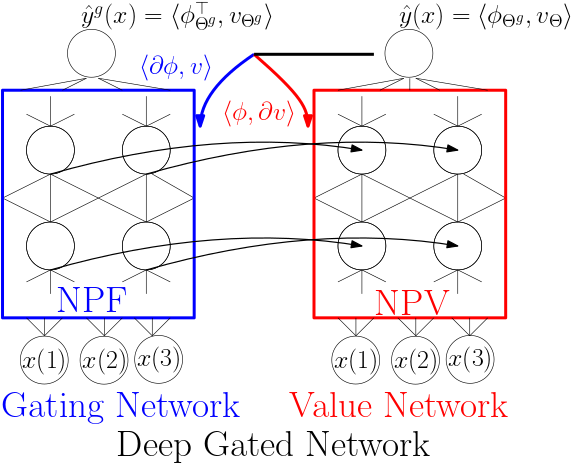
\includegraphics[scale=0.5]{figs/nntwin-blck.png}
}
\end{minipage}
\caption{}
\label{tb:dgn}
\end{table}
\begin{assumption}\label{assmp:main}
(i) $\Theta_0\inrdnet$ is statistically independent of NPFs, (ii) $\Theta_0$ are sampled i.i.d from a distribution such that for any $\theta_0\in\Theta_0$,  we have $\E{\theta_0}=0$, and  $\E{\theta^2_0}=\sigma^2$, and $\E{\theta^4_0}={\sigma'}^2$.
\end{assumption}
\begin{theorem}[\textbf{Main Result}]\label{th:main} Under \Cref{assmp:main}, we have:\\
(i) $\E{K_0}=d\sigma^{2(d-1)} H_0=d\sigma^{2(d-1)} (x^\top x)\odot \lambda_0$.\\
(ii) In addition, if ${4d}/{w^2}<1$, then $Var\left[K_0\right]\leq O\left(d^2_{in}\sigma^{4(d-1)}\max\{d^2w^{2(d-2)+1}, d^3w^{2(d-2)}\}\right)$.
\end{theorem}
\begin{comment}
\begin{lemma}\label{lm:disentangle}[Disentanglement] Let $\nabla_{\Theta} v_t\in \R^{P\times d_{net}}$ be matrix whose entries are given by $\nabla_{\Theta} v_t (p,\theta)=\partial_{\theta}v_t(p),\forall p\in [P], \theta\in\Theta$, and let $I_P$ be the $P\times P$ identity matrix. Then, 
under \Cref{assmp:main}-(ii), it follows that $\E{\nabla_{\Theta}v_{\Theta_t})(\nabla_{\Theta}v_{\Theta_t})^\top }= d\sigma^{2(d-1)}I_{P}$.
\end{lemma}
\begin{comment}
\textbf{Proof of \Cref{th:main}-(i):} Let $\varphi_t=(\varphi_{p,t},p\in[P])\in \R^{d_{net}\times P}$ matrix, then since $K_t=\Psi^\top_t\Psi$, where $\Psi_t=\varphi_t \Phi_t$, we have $\E{K_t}=\E{\Phi^\top_t \varphi^\top_t \varphi_t \Phi_t}$. At initialisation, using the \Cref{assmp:main}-(i), we can pull out $\Phi^\top_t$ and $\Phi_t$ outside of the expectation to have \begin{align}\label{eq:pullout}\E{K_0}=\Phi^\top_0\E{ \varphi^\top_t \varphi_t }\Phi_0,\end{align} and from \Cref{lm:disentangle}, it follows that $\E{ \varphi^\top_t \varphi_t }=d\sigma^{2(d-1)}I$, and hence $\E{K_0}=d\sigma^{2(d-1)}\Phi^\top_0\Phi_0=d\sigma^{2(d-1)}H_0$.\\
\end{comment}
%This overlap is captured by $\lambda_t(s,s')$ which is the measure of overlap of the sub-networks that are active for both the inputs $x,x'\in\R^{d_{in}}$. Under. \Cref{assmp:main}, the inter-path interaction $\varphi^\top_t\varphi_t$ gets disentangled, result in the claim \Cref{th:main}-(i).\\
%However, in the later part of this section, we consider a special case, wherein, we give an explicit characterisation of the spectrum of $\E{K_0}$. Characterising $\lambda_0$ for the general case is left as future work.\\
\textbf{Role of Depth and Width" } Let us first look at the diagonal terms of $\lambda_0$. It is reasonable to assume that, owing to the symmetric nature of the weights, roughly $\mu=\frac{1}{2}$ fraction of the gates are \emph{on} every layer. Thus $\lambda_0(s,s)\approx (w/2)^{d-1}$. Now, due our choice of $\sigma=\sqrt{\frac{2}{w}}$, the diagonal entries will be close to $1$. We now turn our attention towards the non-diagonal entries of $\lambda_0$. Define $\tau(s,s',l)\stackrel{def}=\sum_{i=1}^w G_{x_s,t}(l,i)G_{x_{s'},t}(l,i)$ be the overlap of the active gates in layer $l$ for input examples $s,s'\in[n]$, and  let $\eta\stackrel{def}=\max_s\left(\max_{s',l} \frac{\tau(s,s',l)}{\tau(s,s,l)}\right)$ be the maximum overlap between gates of a layer (maximum taken over over input pairs $s,s'\in[n]$ and layers $l\in [d]$).  Then it follows that $\max_{s,s'\in [n]} \frac{\bar{\lambda}_{cross}(s,s')}{\bar{\lambda}_{self}(s)}\leq \eta^{d-1}$. Thus, the non-diagonal entries decay an exponential rate in comparison to the diagonal entries. The variance expression in \Cref{th:main}-$(ii)$ involves $d^2$ and $d^3$ terms, and hence for a fixed width as depth increases, the entries of $K_0$ deviates from $\E{K_0}$, and as a result the spectrum of $K_0$ degrades, thereby hurting training performance.\\
\textbf{Two random NTFs with identical NPF:}